% !TEX encoding = UTF-8 Unicode 
% !TEX root = praca.tex

\chapter{Literature review}

\section{Related work}

\section{Mobile development relevancy}

\section{Development approaches}

\subsection{Native mobile development}

\subsubsection{Android}
Include Material!!!

\subsubsection{iOS}
Include Cupertino!!!

\subsection{Web development}

\subsection{Cross-platform mobile development}

\subsubsection{Flutter}
\subsubsection{React Native}
\subsubsection{Ionic}
\subsubsection{Comparison}
tutaj tabelka z frameworkami I w kolumnach rozne elementy, np., supported platforms, itd.?

\section{Evaluation of cross-platform frameworks}

\section{Performance measurement}

\subsection{Mobile development}

\subsection{Web development}



% \section{The figure}

% \begin{figure}
% 	\centering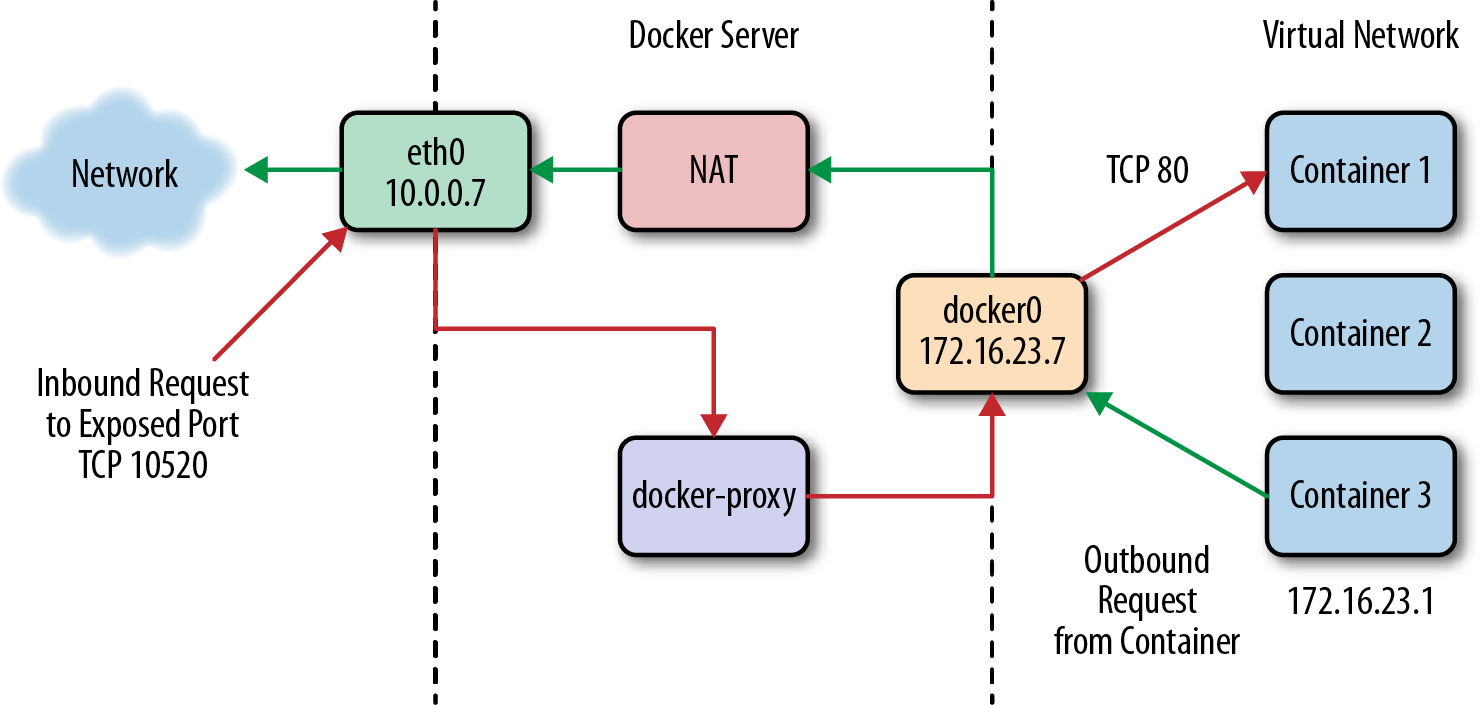
\includegraphics[width=.6\textwidth]{img/swarm-network}
% 	\caption{Docker network \cite{docker_compose_reference}}  \label{rys:network}
% \end{figure}

% In the figure \ref{rys:network} \dots


% \subsection{Two figures side by side}

% \begin{figure}[ht]
% 	\centering
% 	\begin{minipage}[b]{0.45\textwidth}
% 		\centering
\includegraphics[width=0.9\textwidth]{img/kotek} % left figure
% 		\caption{The left figure}\label{fig:lewy}
% 	\end{minipage}
% 	\begin{minipage}[b]{0.45\textwidth}
% 		\centering
% 		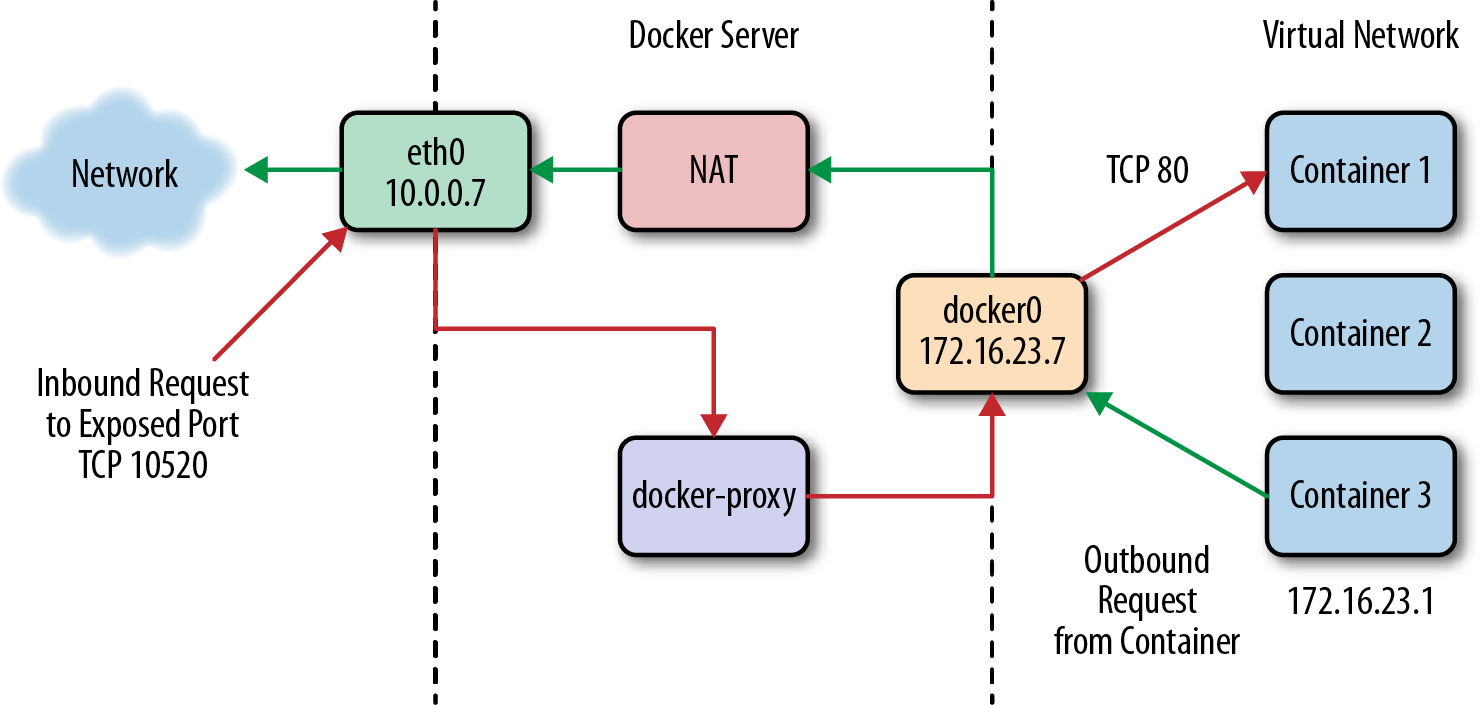
\includegraphics[width=0.9\textwidth]{img/swarm-network} % right figure
% 		\caption{The right figure}\label{fig:prawy}
% 	\end{minipage}
% \end{figure}

% In the figures \ref{fig:lewy} and \ref{fig:prawy} \dots


% \section{The table}

% In the table \ref{table:table1} \dots

% \begin{table}
% 	\centering\caption{The table caption \label{table:table1}}
% 	\begin{tabular}{|l|l|l|}% table alignment -> l c r - left, center, right
% 		\hline
% 		First & Second & Third \\
% 		\hline
% 		First & Second & Third \\
% 		\hline
% 	\end{tabular}
% \end{table}



% \subsection{The equation}

% \begin{equation}
% 	\sum_{i=1}^{\infty}a_i
% 	\label{eq:myEquation}
% \end{equation}

% In the equation \ref{eq:myEquation} \dots


% \section{The listing}

% In the code \ref{listing:myListing} \dots

% % replace {c} with the appropriate language
% \begin{listing}
% 	\begin{minted}{c}  
% int main()
% {
%    int a=2*3;
%    printf("**Ala ma kota\n**");
%    while(!I2C_CheckEvent(I2C1, I2C_EVENT_MASTER_MODE_SELECT)); /* EV5 */
%    return 0;
% }
% \end{minted}
% 	\caption{C language} \label{listing:myListing}
% \end{listing}

